\section{GUI plotting performance}
    We evaluated the performance of the GUI plotting routine. We evaluated the routine when plotting the sampling window observed $\Delta$Q, the mean and confidence bounds of the polling window of observed $\Delta$Qs. 
    \begin{figure}[H]
        \begin{center}
            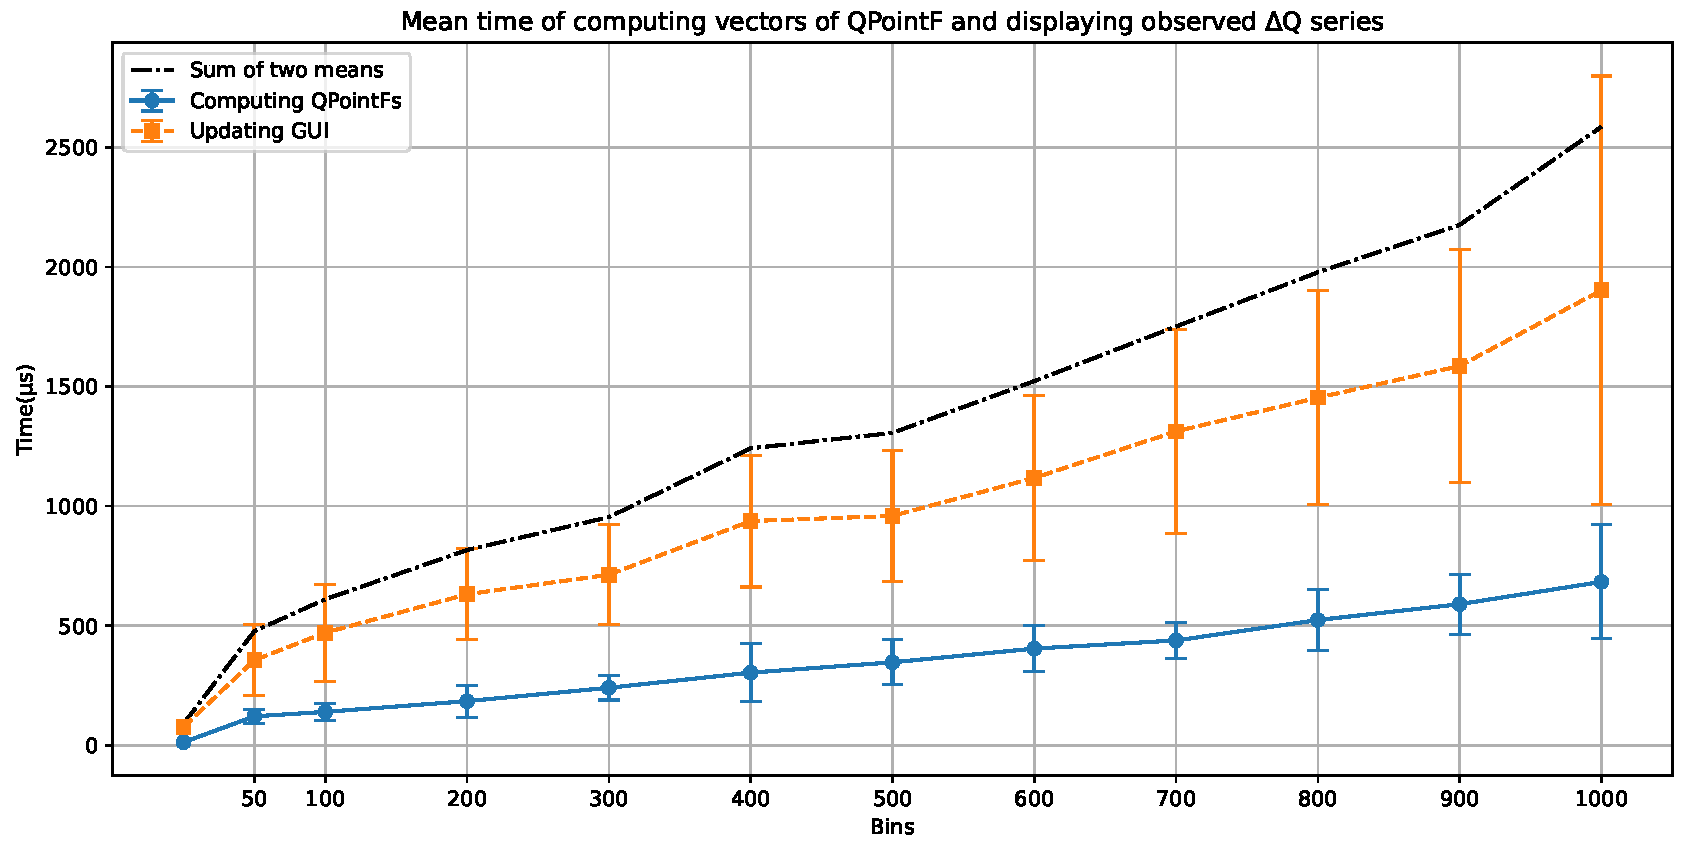
\includegraphics[width = 0.85\textwidth]{img/plots.pdf}
        \end{center}
        \caption{Performance of plotting sampling window and polling window observable $\Delta$Q. \textbf{(Blue, circle)}: QPoinfF vectors setup performance. \textbf{(Orange, square)}: Plotting performance. \textbf{(Black, dotted)}: Sum of the previous two.}
    \end{figure}
    The procedure for preparing and plotting the observed and calculated $\Delta$Q (along with the confidence bounds) is the same, so we would need to double the results we have to obtain the total time for the plot of a sub-outcome diagram.
    The routine first prepares vectors of QPointF \cite{qpointf}, representing all the x and y values of the $\Delta$Qs CDF. The vectors are created for the lower bounds, the upper bounds, the mean of the window of $\Delta$Qs and the observed $\Delta$Q.

    Then, once the vectors are prepared, Qt replaces the old points of a series with the new points for every series being plotted.

    The result scales up to almost 2.5 ms for 1000 bins. We believe that these performances are a big bottleneck of the oscilloscope. If we were to plot the calculated $\Delta$Q and its confidence bounds, the time increase would be twofold. If the sampling rate was 100ms and many probes plots were being displayed, some frames would probably be skipped if the number of bins is high. The high results may nevertheless be explained by the specifications of the PC where we ran the tests, namely by the CPU and the GPU (\cref{app:pc_spec}).
